\documentclass[11pt]{article}
\usepackage[a4paper,left=2cm,right=2cm,top=2cm,bottom=3cm,bindingoffset=5mm]{geometry}
\usepackage[german]{babel}
\usepackage[utf8]{inputenc}
\usepackage{graphicx}
\usepackage{caption}
\usepackage{subcaption}
\usepackage{lastpage}
\usepackage{epstopdf}
\graphicspath{outdir=/u/mhemmer/Documents/Theses/BachelorArbeit/}
\usepackage{fancyhdr}
\usepackage{amsmath}
\usepackage{amsthm}
\usepackage{amsbsy}
\usepackage{amssymb}
\usepackage{hyperref}


\pagestyle{headings}
\fancyhf{}
\setcounter{section}{0}								%Gliederungsnummerierung faengt bei 0 an.

%opening
\title{Systematische Studie der Peakextraktion neutraler Pionen in pp-Kollisionen bei $\sqrt{s}=13\text{ TeV}$ mit Hilfe von Templates}
\author{Marvin Hemmer}

\begin{document}

\maketitle
\newpage
\tableofcontents
\newpage

\section*{Einleitung}

\section{Theoretische Grundlagen}
\subsection{Das Standardmodell der Elementarteilchenphysik}

Es gibt vier Fundamentale Wechselwirkungen: die schwache Wechselwirkung, die starke Wechselwirkung, die elektromagnetische Wechselwirkung und die Gravitation. Das Standardmodell der Elementarteilchenphysik vereint alle bis auf die Gravitation und ist in der Lage die Physik der elementarsten Teilchen damit zu Beschreiben.

Elementarteilchen sind der Grundbaustein jeglicher Materie die bekannt ist und zeichnen sich dadurch aus, dass sie nach aktuellem Wissensstand die kleinsten Teilchen sind. Anders ausgedrückt, Elementarteilchen sind nicht weiter teilbar in andere Teilchen.

Diese Elementarteilchen wechselwirken miteinander aufgrund ihrer Ladung(en). Das Elektron z.B. hat eine elektrische Ladung von $-1$. Durch die elektrische Ladung ist es in der Lage an elektromagnetischer Wechselwirkung teilzunehmen. Wenn zwei Teilchen miteinander wechselwirken, dann geschieht das unter Austausch eines sogenannten Austauschteilchens, im Falle der elektromagnetischen Wechselwirkung durch Austausch eines Photons.

Die Elementarteilchen kann man nun entsprechend ihrer elektrischen Ladung und der Generation unterteilen. Ebenso lassen sich die Austauschteilchen ihrer entsprechenden Wechselwirkung zuordnen, wobei diese ebenfalls zu den Elementarteilchen z{\"a}hlen. Dies wurde in den beiden Tabellen \ref{tab:teilchen} und \ref{tab:Austeilchen} gemacht. Es gibt also sechs Quarks und sechs Leptonen, mit jeweils ihren entsprechend Antiteilchen.

\begin{table}[h] 
\centering
\begin{tabular}{|c||c|c|c||c|}
\hline
Generation & I                                                                                    & II                                                                              & III                                                                             & el. Ladung                                           \\ \hline \hline
Quarks    & \begin{tabular}[c]{@{}c@{}}up ($u$)\\ down ($d$)\end{tabular}                        & \begin{tabular}[c]{@{}c@{}}charm ($c$)\\ strange ($s$)\end{tabular}             & \begin{tabular}[c]{@{}c@{}}top ($t$)\\ bottom ($b$)\end{tabular}                & \begin{tabular}[c]{@{}c@{}}+2/3\\  -1/3\end{tabular} \\ \hline
Leptonen  & \begin{tabular}[c]{@{}c@{}}Elektron ($e$)\\ Elektron-Neutrino ($\nu_{e}$)\end{tabular} & \begin{tabular}[c]{@{}c@{}}Myon($\mu$)\\ Myon-Neutrino ($\nu_{\mu}$)\end{tabular} & \begin{tabular}[c]{@{}c@{}}Tau($\tau$)\\ Tau-Neutrino ($\nu_{\tau}$)\end{tabular} & \begin{tabular}[c]{@{}c@{}}-1\\  0\end{tabular}      \\ \hline
\end{tabular}
\caption{Tabelle der Elementarteilchen}
\label{tab:teilchen}
\end{table}


\begin{table}[h]
\centering
\begin{tabular}{|c||c|c|c|}
\hline
Wechselwirkung    & elektromagnetisch & stark       & schwach                      \\ \hline
Austauschteilchen & Photon ($\gamma$) & Gluon ($g$) & $W^{\pm}$, $Z^{0}$ - Bosonen \\ \hline
\end{tabular}
\caption{Tabelle der Austauschteilchen}
\label{tab:Austeilchen}
\end{table}

Zus\"atzlich zu den bisher genannten Gr\"o{\ss}en lassen sich den Elementarteilchen noch weitere Eigenschaften zuschreiben. So haben alle drei Austauschteilchen einen Spin von $1$ und geh\"ohren somit zu den Bosonen. Quarks und Leptonen tragen hingegen einen Spin von $1/2$ und geh\"ohren entsprechend zu den Fermionen.

Wie oben bereits erw\"ahnt koppeln Kr\"afte an die Ladung von Teilchen. Um die elektromagnetische Kraft zu Beschreiben gibt es die Quantenelektrodynamik (QED). F\"ur die starke Wechselwirkung gibt es entsprechend die Quantenchromodynamik (QCD). Der Name kommt daher, dass die Ladung, die zur starken Wechselwirkung geh\"ohrt, die Farbladung ist (chroma ist griechisch für Farbe). Die Farbladung hat dabei nichts mit der \"au{\ss}eren Erscheinung der Quarks zu tun.

\subsection{Starke Wechselwirkung und das Quark-Gluon-Plasma}
Die starke Wechselwirkung ist für die Bindung von Quarks verantwortlich. Durch die starke Wechselwirkung gebundene Zust\"ande hei{\ss}en hadronen. Dabei gibt es zwei M\"oglichkeiten, wie sich Quarks binden k\"onnen. Zum einen bilden drei Quarks ($qqq$) ein Baryon und ein Quark mit einem Antiquark ($q\bar{q}$) ein Meson. Neben Baryonen gibt es auch entsprechende Antiteilchen, welche aus drei Antiquarks bestehen ($\bar{q}\bar{q}\bar{q}$).

Die zwei bekanntesten Baryonen hei{\ss}en Proton ($uud$) und Neutron ($udd$). Protonen und Neutronen die den Atomkern bilden sind also anders als die Elektron, die um den Atomkern kreisen, nicht elementar.

Wie bereits zuvor angesprochen tragen Quarks eine gewisse Farbladung. Die g\"annigste Bennenung der drei (Anti-)Farben ist rot, blau und gr\"un, in Anlehnung an die Farblehre, da eine Kombination aller drei Farben wei{\ss} ergibt. Ebenso ergibt Farbe und entsprechende Antifarbe auch wei{\ss}.
Mesonen oder Baryonen sind jedoch farbneutral nach au{\ss}en hin.
Anders als in der elektromagnetischen Wechselwirkung die Photonen, tragen die Gluonen als Austauschteilchen ebenfalls Farbladung und können somit auch selbst wechselwirken.

Die Kraft die auf farbgeladene Teilchen wirkt folgt aus einem Potential $V(r)$. F\"ur dieses Potential gilt:
\begin{align} \label{eq:Potential}
V(r) = -\frac{4}{3}\frac{\alpha_\text{s}}{r} + kr
\end{align}
$\alpha_\text{s}$ bezeichnet die Kopplungskonstante der starken Wechselwirkung. Der anziehende Teil des Potentials ist also proportional zum Abstand der beiden farbgeladenen Teilchen, w\"ahrend der absto{\ss}ende Teil mit zunehmendem Abstand kleiner wird. Anders als in der QED wird die Anziehung zweier Teilchen also immer stärker je weiter man sie von einander entfernt. Die Feldlinien verdichten sich und durch die zuvor angesprochene M\"oglichkeit von Gluonen miteinander zu wechselwirken, verbinden sich die Feldlinien. Eine solche Kette von Feldlinien bezeichent man auch als \textit{string}. 

Wenn man zwei Teilchen weit genug von einander entfernt ist die benötigte Energie um sie weiter voneinander zu entfernen so gro{\ss}, dass es zum sogenannten \textit{stringbreaking} kommt und ein neues Teilchen Antiteilchen Paar entsteht. Dies ist möglich nach der \"Aquivalenz von Masse und Energie wie sie 1905 von Albert Einstein entdeckt wurde.

Das hat zur Folge, dass es in der Natur keine freien Teilchen mit Farbladung gibt. Dieses Verhalten nennt man \textit{confinement}.

Um die starke Wechselwirkung und die Quarks und Gluonen untersuchen zu k\"onnen muss dieses confinement aufgebrochen werden. Dabei spielt die Kopplungskonstante $\alpha_\text{s}$ eine Rolle. Anders als die Bezeichnung vermuten l\"asst ist sie n\"amlich nicht konstant. Stattdessen h\"angt $\alpha_\text{s}$ vom Impulsübertragsquadrat $Q^{2}$ zwischen zwei Teilchen ab. Aufgrund dieses Zusammenhangs nennt man die Wechselwirkung auch \textit{running coupling}. 

Das Impulsübertragsquadrat $Q^{2}$, bzw. der Impulsübertrag $Q$ h\"angt dabei selbst \"uber die De-Broglie-Wellenl\"ange mit dem Abstand $r$ zusammen. Es gilt $Q = \frac{h}{\lambda}$, wobei $\lambda$ die r\"aumliche Aufl\"osung beschreibt. F\"ur eine genau Aufl\"osung, also f\"ur  sehr kleine $r$ muss $Q$ gro{\ss} sein.
Zusammengefasst h\"angt $\alpha_\text{s}$ also von $r$ an. Dabei ist $\alpha_\text{s}(r)$ klein f\"ur kleine $r$, bzw. gro{\ss}e $Q$.
Wenn $\alpha_\text{s}$ klein genug wird k\"onnen Quarks und Gluonen theoretisch frei beobachtet werden. Dieser Verlauf von $\alpha_\text{s}$ wird Asymptotische Freiheit genannt. Einen Zustand in dem Quarks und Gluonen sich quasi frei bewegen k\"onnen nennt man Quark-Gluonen-Plasma.

\subsection{Messung neutraler Mesonen}

\section{Experimenteller Aufbau}
\subsection{CERN}
\subsection{LHC}
\subsection{ALICE}
\subsection{Das elektromagnetische Kaloriemeter}

\section{Analyse}
\subsection{Daten}
\subsubsection{Datensatz} \label{ssec:Datensatz}
\subsubsection{Trigger und Clusterauswahlkriterien}
\subsection{Peak Extraktion mit Hilfe von Parametrisierungen von Funktionen}
\subsubsection{Rekonstruktion neutraler Pionen}

Messungen mit dem EMCal liefern Information {\"u}ber Ort und Energie von unter anderem Photonenkandidaten. Mit diesen Informationen k{\"o}nnen ${\it \pi^{0}}$ rekonstruiert werden, da ein ${\it \pi^{0}}$ zu $\left( 98,823\pm0,034\right)\%$ [QUELLE PDG] in zwei Photonen zerf{\"a}llt. Ein ${\it \pi^{0}}$ zerf{\"a}llt nach einer mittleren Wegl{\"a}nge von ${\it c\tau} = 25,5$nm vom prim{\"a}ren Vertex. Der prim{\"a}re Vertex wird mit Hilfe des ITS bestimmt. \\
Mit dem Wissen, wo sich der prim{\"a}ren Vertex befindet, sowie der Ortsmessung des EMCals, kann der Zerfallswinkel $\theta_{\gamma\gamma}$ zwischen zwei Photonenkandidaten, die mit dem EMCal detektiert wurden, bestimmt werden. \\ 
Um die invariante Masse $m_{\text{inv}}$ zu berechnen, sind die Energien $E_{\gamma1}$ und $E_{\gamma2}$ der beiden Photonenkandidaten, sowie der Zerfallswinkel $\theta_{\gamma\gamma}$ erforderlich. \\
Die Zahlen in den Indizes beziehen sich dabei auf die Nummerierung der beiden Photonen. Die Indizes x und y beziehen sich auf die Raumrichtungen. F{\"u}r diese gilt:
\begin{align}
m_{\text{inv}} &= \sqrt{2E_{\gamma\it{1}}E_{\gamma\it{2}}(1-\cos\left( \theta_{\gamma\gamma}\right) )} \label{eq_invmass}
\end{align}
Au{\ss}erdem kann die Aufteilung des Impulses der Photonenkandidaten bestimmt werden, die wiederum notwendig ist, um den Transversalimpuls $p_{T}$ des $\pi^{0}$ zu Berechnen. Es gilt:
\begin{align}
p_{T\pi^{0}} &= \sqrt{\left(p_{x1}+p_{x2}\right)^{2} +\left(p_{y1}+p_{y2}\right)^{2}} \label{eq_pt}
\end{align}
\begin{figure}[tbp] \label{figInvMassPt}
	\centering
	\begin{subfigure}{.5\textwidth}
		\centering
		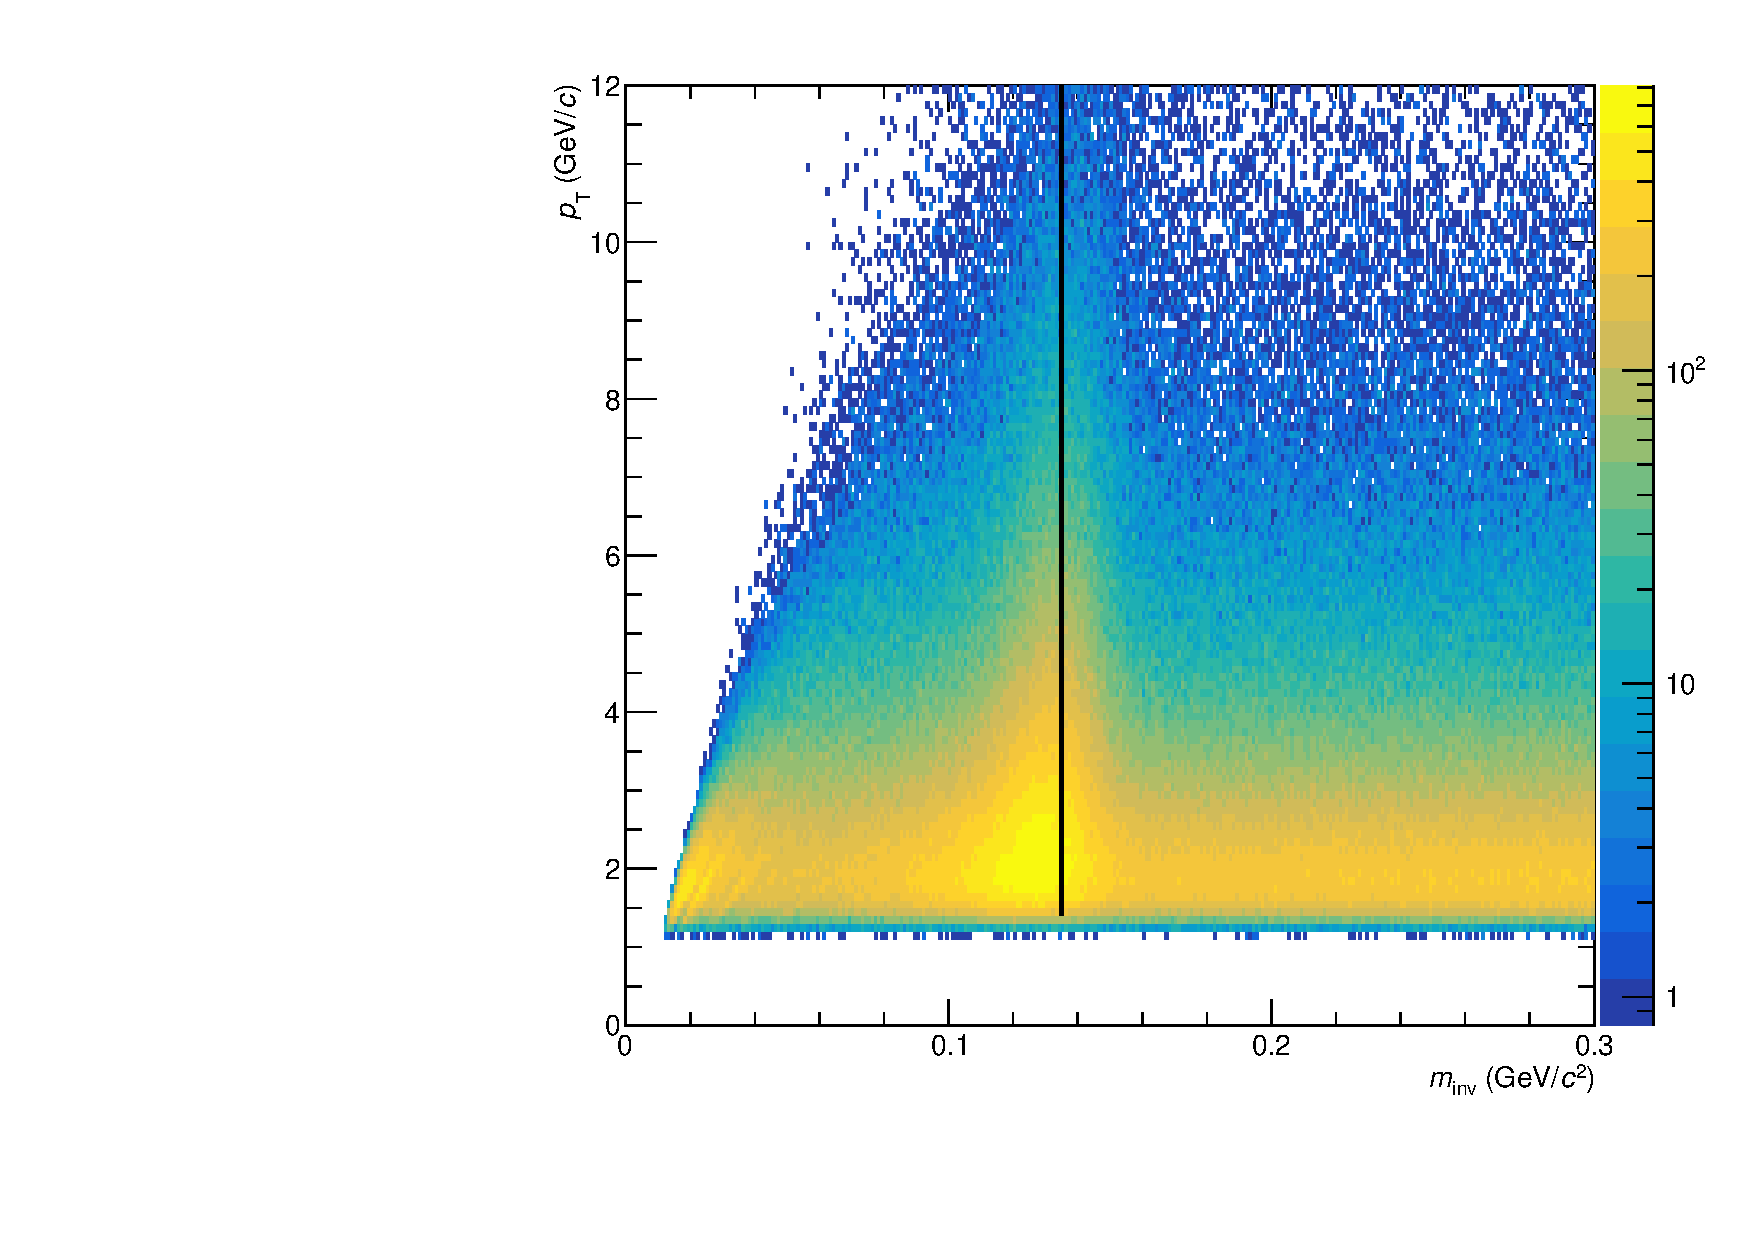
\includegraphics[width=.95\linewidth]{hInvMass_pT_Signal.pdf}
		\caption{}
		\label{figInvMassPt_a}
	\end{subfigure}%
	\begin{subfigure}{.5\textwidth}
		\centering
		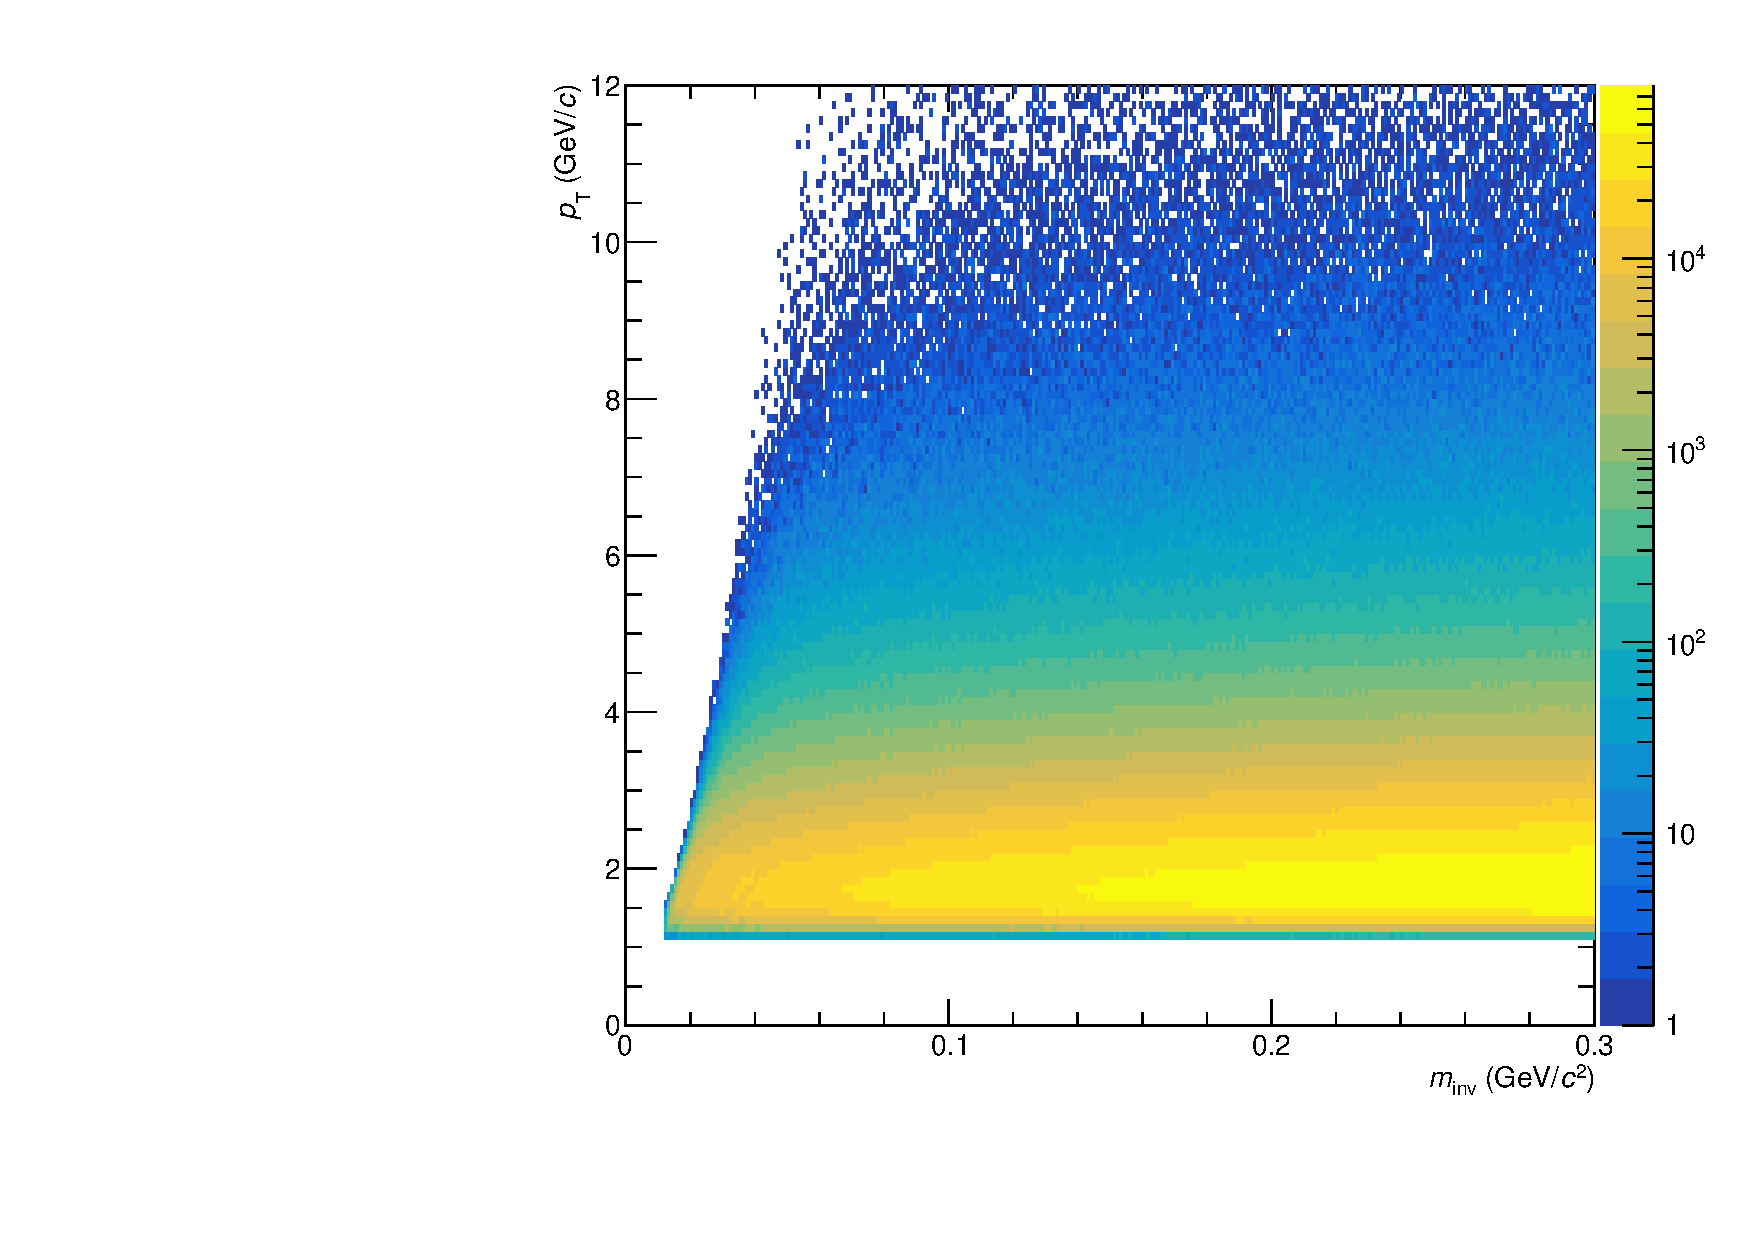
\includegraphics[width=.95\linewidth]{hInvMass_pT_Bkg.pdf}
		\caption{}
		\label{figInvMassPt_b}
	\end{subfigure}
	\caption{\newline{\bf (a)}: $p_\text{T}$ und $m_\text{inv}$ als Funktion von der Anzahl von rekombinierten  Cluster-Paaren aus der gleichen Kollision. Die schwarze Linie liegt bei $m_{\text{inv}}=0,135\text{ GeV/}c^{2}$, was der $\pi^{0}$ Masse entspricht, wo eine deutliche Peakstruktur zu Erkennen ist.\newline{\bf (b)}: $p_\text{T}$ und $m_\text{inv}$ als Funktion von der Anzahl von rekombinierten  Cluster-Paaren aus unterschiedlichen Kollision.}
\end{figure}
Aus dem in Abschnitt \ref{ssec:Datensatz} erw{\"a}hnten Datensatz werden alle m{\"o}glichen Kombinationen von zwei Photonenkandidaten aus der gleichen Kollision benutzt, um $m_{\text{inv}}$ nach Gleichung \ref{eq_invmass} zu berechnen. Diese Methode wird auch als {\it same event} bezeichnet. Au{\ss}erdem wird $p_{T,\pi^{0}}$ nach Gleichung \ref{eq_pt} berechnet um aus den $m_{\text{inv}}$ und $p_{T,\pi^{0}}$ Wertepaaren eine invariante Massenverteilung zu erhalten. In Abbildung \ref{figInvMassPt_a}) ist die invariante Massenverteilung des Datensatzes zu sehen. In dieser Verteilung sticht eine h{\"a}ufung der Datenpunkte bei $m_{\text{inv}}\approx 0,135\text{GeV/}c^{2}$ heraus. Abbildung \ref{figInvMassPt_b} zeigt die invariante Massenverteilung bei der Photonenkandidaten aus unterschiedlichen Kollisionen miteinander kombiniert werden. Diese Methode wird als {\it mixed event} bezeichnet. Auf die Verteilung wird in Kapitel \ref{sssec:num3} genauer eingegangen.

	\begin{figure}[tbp]
		\centering
		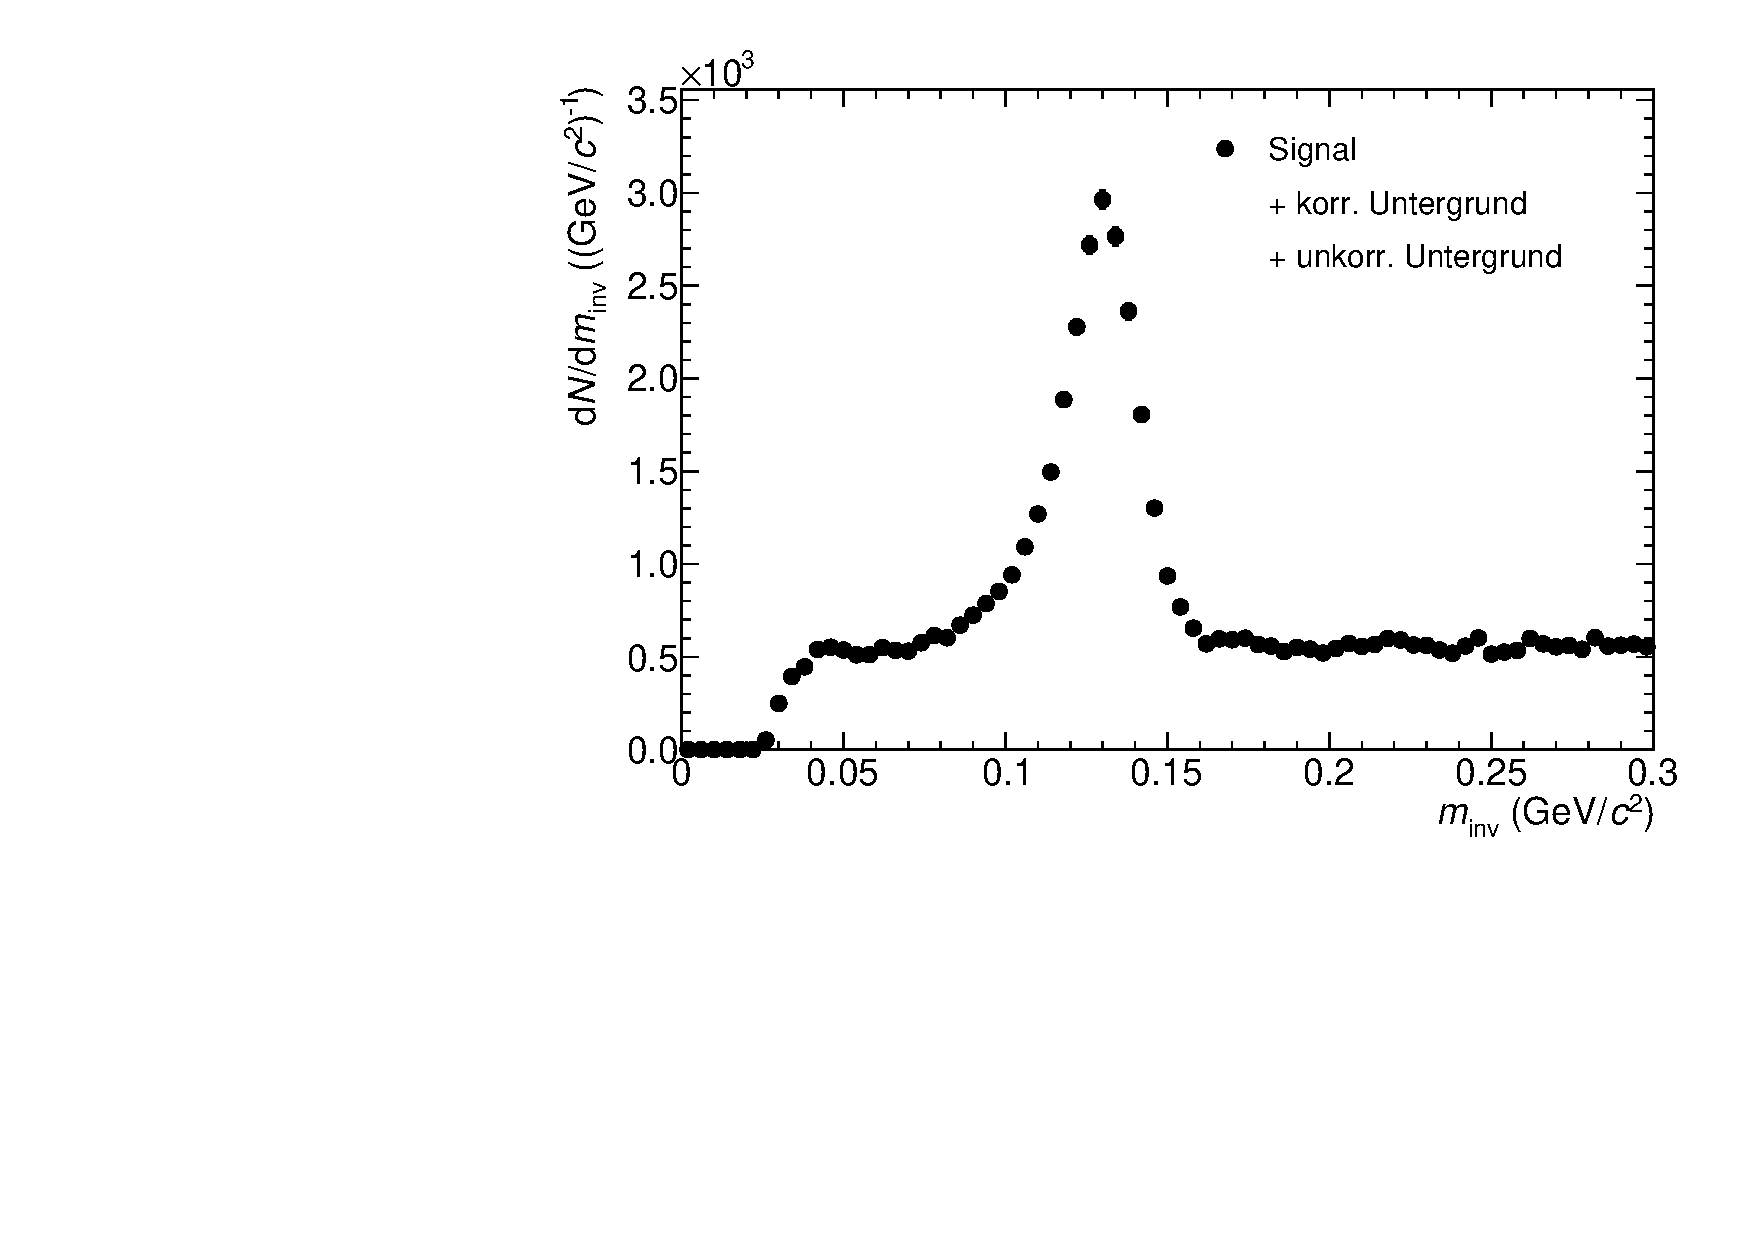
\includegraphics[width=.7\linewidth]{hSignalPlusBkg.pdf}
		\caption{Projektion von Abbildung \ref{figInvMassPt_a} im $p_{\text{T}}$-Intervall (3.2 - 3.4) $(\text{GeV/}c)$. Es ist ein deutlicher Peak um $m_{\pi^{0}} \approx 0,135\text{GeV/}c^{2}$ zu erkennen, aber auch Untergrund, da das Signal zu h{\"o}heren Massen gau{\ss}f{\"o}rmig abklingen sollte. Bei $m_{\text{inv}} < m_{\pi^{0}}$ kann Signal vorliegen, das aus konvertierten Photonen besteht, weshalb eine Aussage {\"u}ber die Form, bzw. den Untergrund dort schwer m{\"o}glich ist.}
		\label{figSignalPlusBkg}
	\end{figure}

	Um $\pi^{0}$s in einzelnen $p_{T}$-Intervallen z{\"a}hlen zu k{\"o}nnen wird die Verteilung in entsprechende Abst{\"a}nden auf die Y-Achse projiziert. Die Intervalle werden so gew{\"a}hlt, dass sie m{\"o}glichst klein sind, w{\"a}hrend die statistischen Unsicherheiten nicht zu gro{\ss} werden. Man erh{\"a}lt Verteilungen der invarianten Masse, die aus Signal, sowie korreliertem und unkorreliertem Untergrund bestehen (vgl. Abbildung \ref{figSignalPlusBkg}). Dennoch ist ein deutlicher Peak im Bereich der Pionenmasse von ca. 135MeV/$c^{2}$ zu erkennen. Um das Signal zu extrahieren werden im Folgende die beiden Komponenten des Untergrunds pr{\"a}sumiert.

	\subsubsection{Absch{\"a}tzung des unkorrelierten Untergrunds}
	\label{sssec:num3}

	\begin{figure}[tbp]
		\centering
		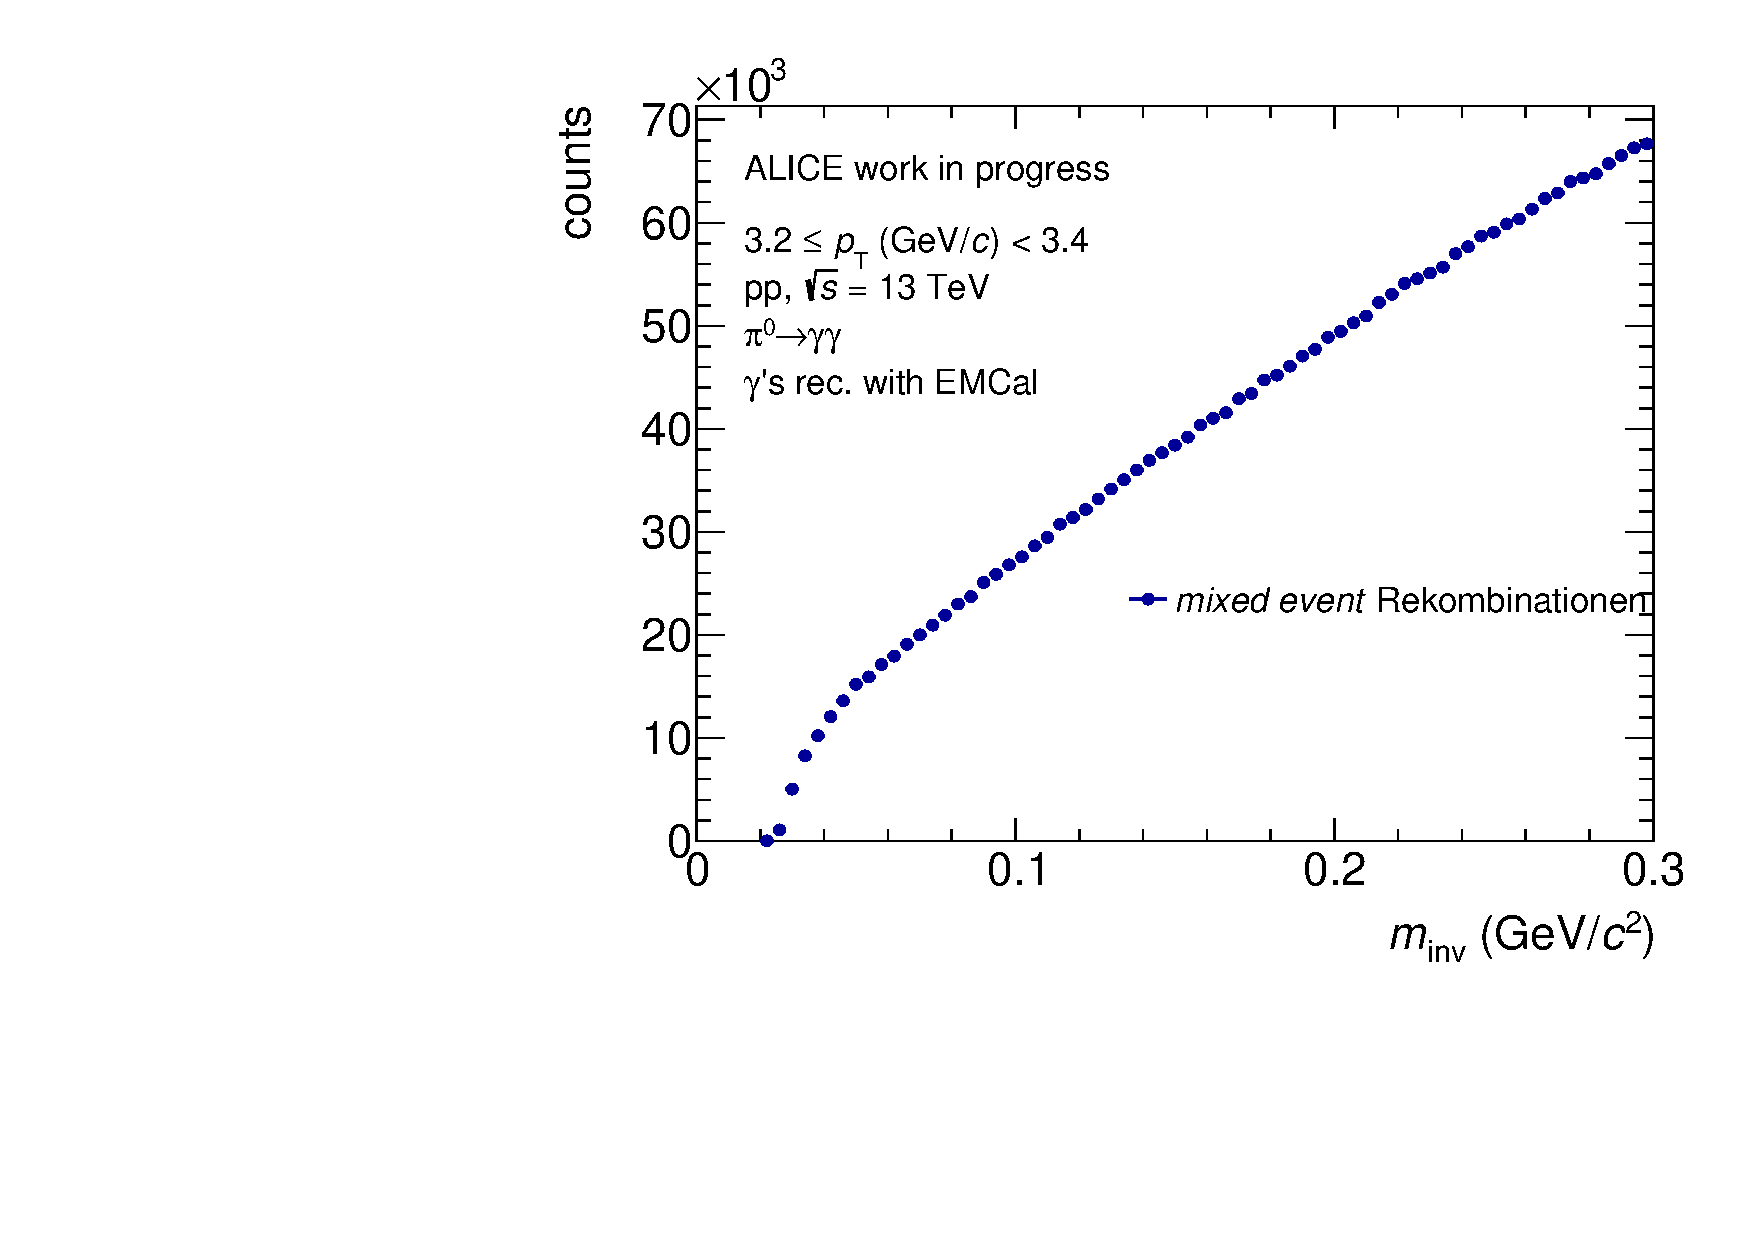
\includegraphics[width=.7\linewidth]{hUncorrBkg.pdf}
		\caption{Kombinationen von Photonenkandidaten aus unterschiedlichen Kollisionen, die keine Korrelationen zueinander haben, weshalb auch kein Peak im Bereich der $\pi^{0}$-Masse zu sehen ist. Dies dient als Grundlage zur Bestimmung des unkorrelierten Untergrunds.}
		\label{figUncorrBkg}
	\end{figure}

	Durch das kombinieren aller Photonenkandidaten ist ein gro{\ss}er Anteil der rekonstruierten Massen aus nicht korreliert Paaren, da die beiden Photonenkandidaten nicht zusammenh{"a}ngen {\"u}ber beispielsweise einen Zerfall. Um diesen unkorrelierten Untergrund abzuw{\"a}gen kombiniert man im sogenannten Eventmixing Photonenkandidaten aus unterschiedlichen Events zusammen, da so sicher keine Verbindung zwischen den beiden Photonenkandidaten besteht. Abbildung \ref{figUncorrBkg} stellt das Ergebnis des Eventmixings f{\"u}r einen gew{\"a}hlten Bereich dar.

	Die Verteilung aus den {\it mixed events} weist keinen Peak auf und hat eine gr{\"o}{\ss}ere Anzahl Eintr{\"a}ge, als die Verteilung aus dem selben Events (vgl. Abbildung \ref{figSignalPlusBkg} und \ref{figUncorrBkg}), weshalb die mixed Event Verteilung an die der same Events skaliert werden muss. Die Skalierung erfolgt im rechten Bereich au{\ss}erhalb des $\pi^{0}$-Peaks und es ergibt sich f{\"u}r den Skalierungsfaktor:
	\begin{align}
	\label{eqBackSkalierung}
	\alpha &= \frac{\sum_{i \neq j}\sum_{n}m_{\text{inv}}\left( \gamma^{(n)}_{i},\gamma^{(n)}_{j}\right) }{\sum_{i,j}\sum_{n \neq m}m_{\text{inv}}\left( \gamma^{(n)}_{i},\gamma^{(m)}_{j}\right) }
	\end{align}
	Die oberen Indizes stehen hierbei f{\"u}r das Event, aus dem ein Photon kommt.\newline
	\begin{figure}[tbp]
		\centering
		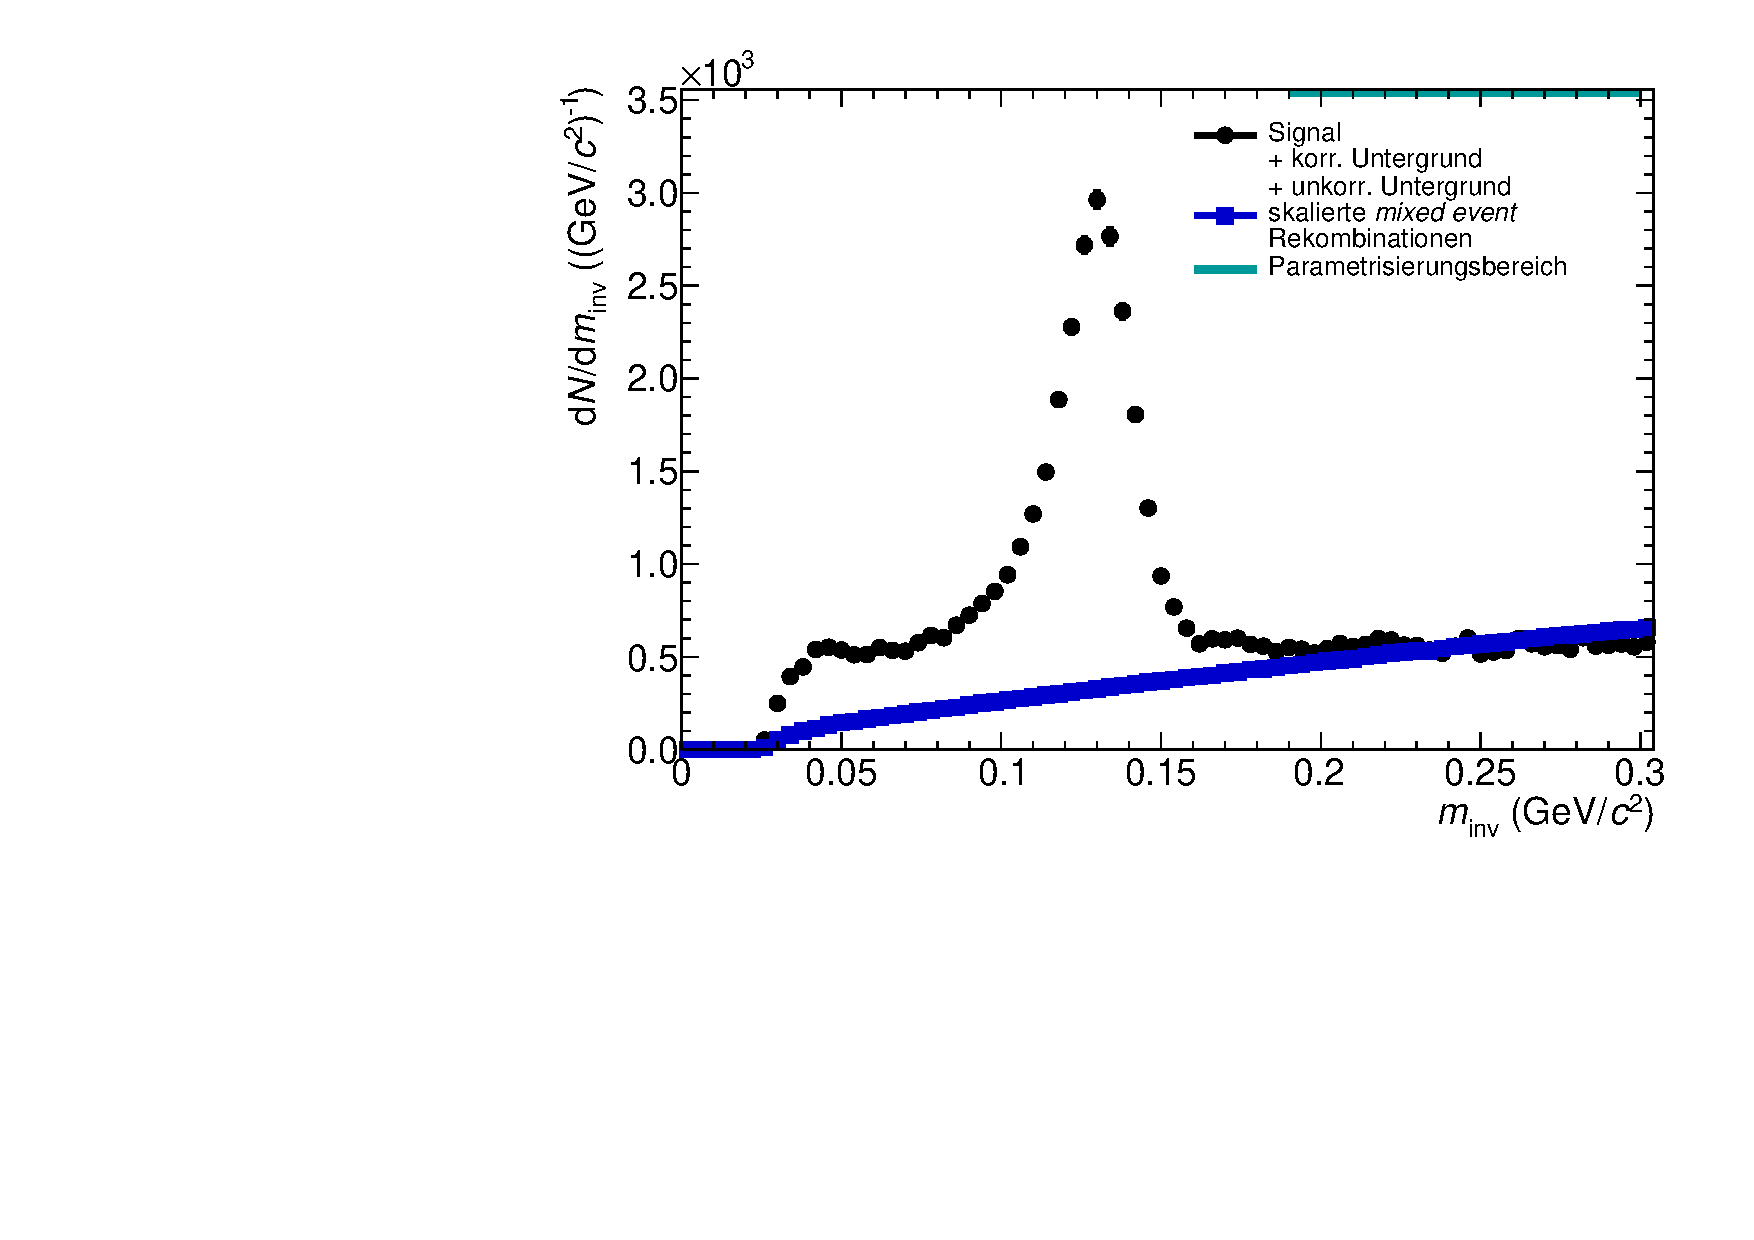
\includegraphics[width=.7\linewidth]{hUncorrBkgNorm.pdf}
		\caption{Nach Gleichung \ref{eqBackSkalierung} skalierte {\it mixed event} Rekombinationen aus Abbildung \ref{figUncorrBkg} als Absch{\"a}tzung des unkorrelierten Untergrunds zusammen aufgetragen mit Signal zuz{\"u}glich beiden Untergrundkomponenten (Abbildung \ref{figSignalPlusBkg}).}
		\label{figUncorrBkgNorm}
	\end{figure}
	Das Resultat der Skalierung ist in Abbildung \ref{figUncorrBkgNorm} zu sehen, wo zus{\"a}tzlich noch das Signal inklusiver beider Untergr{\"u}nde eingezeichnet ist, um besser erkennen zu k{\"o}nnen, wie sich der abgesch{\"a}tzte korrelierte Untergrund relativ zum gesamten Signal verh{\"a}lt.
	Das es sich hierbei nur um eine Absch{\"a}tzung handelt kann daran ausmachen werden, dass um $m_{\text{inv}} = 0,3 (\text{GeV/}c)$ der unkorrelierte Untergrund gr{\"o}{\ss}er ist, als das Signal mit beiden Untergrundkomponenten, was bedeutet, dass nach Abzug des unkorrelierten Untergrunds das Signal mit korreliertem Untergrund dort negativ w{\"a}re, was physikalisch nicht sinnvoll ist.
	\subsubsection{Absch{\"a}tzung des korrelierten Untergrunds}
	\subsection{Peak Extraktion mit Hilfe von Parametrisierungen von Templates}
	\subsubsection{Templates}
	\subsubsection{Fit Methode}
\section{Korrigierter Yield}
\subsection{Korrekturen}
\subsection{Variationen}
\section{Zusammenfassung und Aussicht}



\end{document}
